% ============================================================
%  Market Calibration of the CGMY Process to SPX Options
%  Full calibration report — methodology, data, and results
% ============================================================
\documentclass[11pt,a4paper]{article}

\usepackage{amsmath,amssymb,amsthm}
\usepackage{booktabs}
\usepackage{graphicx}
\usepackage{hyperref}
\usepackage{geometry}
\usepackage[expansion=false]{microtype}
\usepackage{caption}
\usepackage{subcaption}
\usepackage{parskip}
\usepackage{xcolor}
\usepackage{array}
\usepackage{multirow}
\usepackage{enumitem}
\usepackage{tabularx}
\usepackage{siunitx}

\geometry{top=2.5cm, bottom=2.5cm, left=2.8cm, right=2.8cm}

\hypersetup{
  colorlinks=true,
  linkcolor=blue!60!black,
  citecolor=blue!60!black,
  urlcolor=blue!60!black,
}

\captionsetup{font=small, labelfont=bf, skip=6pt}

\newcommand{\E}{\mathbb{E}}
\newcommand{\R}{\mathbb{R}}
\newcommand{\vp}{\text{vp}}     % vol-points abbreviation

% ─────────────────────────────────────────────────────────────────────────────
\title{%
  \textbf{Market Calibration of the CGMY Tempered Stable Process\\
  to SPX Implied-Volatility Surfaces}\\[0.5em]
  \large Methodology, Implementation, and Results
}
\author{Davood Damircheli}
\date{\today}

\begin{document}
\maketitle

% ── Abstract ─────────────────────────────────────────────────────────────────
\begin{abstract}
We calibrate the four-parameter
Carr--G\'{e}man--Madan--Yor (CGMY) tempered stable L\'{e}vy model
to S\&P~500 (SPX) implied-volatility (IV) surfaces on three dates spanning
distinct market regimes: a pre-COVID low-volatility period (January 2020),
the acute COVID-19 crisis (March 2020), and the post-COVID recovery
(September 2021).
The inner pricing engine is a B-Spline Galerkin + Crank--Nicolson solver
for the fractional backward FPDE; a two-phase Differential Evolution plus
L-BFGS-B optimizer calibrates all four parameters in under five minutes per
date on a single CPU core.
On well-identified surfaces (five maturities, tight bid-ask spreads)
the in-sample IV RMSE is 1.97--2.47 vol-points.
The crisis date, where the 5\,\% spread filter retains only two maturities,
yields 7.19 vol-points — a data-quality limitation rather than an algorithmic
failure.
Cross-regime analysis confirms that the fine-structure index $Y^*$ is stable
(range 3.6\,\% of the cross-date mean), while the jump-intensity parameter
$C^*$ is 5.6--11$\times$ elevated at the crisis date.
An accuracy-matched comparison against a Gr\"{u}nwald--Letnikov
finite-difference solver shows GL calibration completes in 20\,s versus
115\,s for the B-spline, driven by GL's zero pre-build cost and a 6.7$\times$
cheaper per-evaluation, though the B-spline retains a decisive accuracy
advantage ($O(h^{2.5})$ vs.\ $O(h)$) that makes it the preferred choice at
high-accuracy requirements.
\end{abstract}

\tableofcontents
\listoffigures
\listoftables
\clearpage

% =============================================================================
\section{Introduction}
\label{sec:intro}
% =============================================================================

Fitting a parametric model to a full option surface is a standard step in
quantitative finance: it extracts the market-implied risk-neutral distribution,
enables consistent pricing across strikes and maturities, and tests whether the
model's structural assumptions are consistent with observable prices.
The CGMY model (Carr, Géman, Madan \& Yor, 2002) is a natural candidate for SPX options because its
L\'{e}vy measure
\[
  k(x) = C\,\frac{e^{-M x}}{x^{1+Y}}\,\mathbf{1}_{x>0}
        + C\,\frac{e^{-G|x|}}{|x|^{1+Y}}\,\mathbf{1}_{x<0}
\]
can simultaneously capture heavy tails ($Y$ close to 2), negative skew
(asymmetric $G \neq M$), and a controllable activity level ($C$) with only
four parameters.

The two main computational challenges are:
\begin{enumerate}[leftmargin=*]
  \item \textbf{Pricing speed.} Each optimizer call must price all strikes
        across all maturities.  The CGMY fractional FPDE involves a dense,
        non-local operator; a naive assembly and solve per optimizer call would
        take minutes per surface evaluation.
  \item \textbf{Global search.} The vega-weighted loss surface is multi-modal;
        local gradient methods converge to the wrong basin from a generic
        starting point.
\end{enumerate}

This report documents the end-to-end solution to both challenges, using the
B-Spline Galerkin + CN solver as the pricing engine and a two-phase
Differential Evolution + L-BFGS-B optimizer.
The pipeline is applied to three snapshot dates that represent markedly
different market regimes:
\begin{itemize}
  \item \textbf{2020-01-15} — low-volatility environment (VIX $\approx 13$,
        pre-COVID).
  \item \textbf{2020-03-18} — acute COVID-19 crisis (VIX $\approx 76$,
        extreme intraday moves, severely dislocated bid-ask spreads).
  \item \textbf{2021-09-15} — post-COVID recovery (VIX $\approx 20$,
        ample liquidity).
\end{itemize}

The report is structured as follows.
Section~\ref{sec:model} recalls the CGMY model.
Section~\ref{sec:data} describes the data pipeline and quality filters.
Section~\ref{sec:pricing} details the pricing engine and the caching
architecture that makes calibration tractable.
Section~\ref{sec:calib_method} presents the calibration methodology.
Section~\ref{sec:results} reports the numerical results, figures, and timing.
Section~\ref{sec:interp} discusses the financial interpretation.
Section~\ref{sec:robustness} performs the crisis-date robustness check.
Section~\ref{sec:crisis_caveat} analyses the crisis fit caveat.
Section~\ref{sec:gl_benchmark} presents the Gr\"{u}nwald--Letnikov
speed benchmark.
Section~\ref{sec:conclusion} concludes.

% =============================================================================
\section{The CGMY Model}
\label{sec:model}
% =============================================================================

\subsection{Characteristic exponent}

The CGMY L\'{e}vy process $X = (X_t)_{t \ge 0}$ is defined by its
characteristic exponent
\begin{equation}
  \Psi(u) \;=\; C\,\Gamma(-Y)\bigl[
    (M - iu)^{Y} - M^{Y}
    + (G + iu)^{Y} - G^{Y}
  \bigr],
  \qquad u \in \R,
  \label{eq:cgmy_cf}
\end{equation}
so that $\E[e^{iuX_t}] = e^{t\,\Psi(u)}$.  The four parameters are:
\begin{itemize}[noitemsep]
  \item $C > 0$: overall jump intensity (scales the L\'{e}vy measure).
  \item $G > 0$: left-tail exponential decay rate.
  \item $M > 1$: right-tail exponential decay rate
        ($M > 1$ ensures $\E[e^{X_1}] < \infty$, i.e.\ finite stock price).
  \item $Y \in (0,2)\setminus\{1\}$: fine-structure index; for $Y \in (1,2)$
        the process has infinite variation, which is the relevant regime
        for equity L\'{e}vy models.
\end{itemize}

\subsection{Risk-neutral dynamics}

Under the risk-neutral measure $\mathbb{Q}$, the log-price process is
\begin{equation}
  \log(S_T / S_0) \;=\; (r - q - \omega_S)\,T + X_T,
  \label{eq:log_price}
\end{equation}
where $r$ is the continuously-compounded risk-free rate, $q$ is the dividend
yield, and the martingale correction
\begin{equation}
  \omega_S \;=\; C\,\Gamma(-Y)\,
  \bigl[(M-1)^Y - M^Y + (G+1)^Y - G^Y\bigr]
  \label{eq:omega}
\end{equation}
ensures $\E_\mathbb{Q}[S_T] = S_0\,e^{(r-q)T}$.

% =============================================================================
\section{Data and Surface Construction}
\label{sec:data}
% =============================================================================

\subsection{Raw data}

Raw option chains are sourced from OptionMetrics for the three snapshot dates.
Each chain contains end-of-day bid price, ask price, and implied volatility
for all listed SPX European calls and puts across all available strikes and
maturities.

\subsection{Step 1 — quality filters}

The following filters are applied to each raw chain before any further
processing:
\begin{enumerate}[leftmargin=*, label=(\roman*)]
  \item Remove quotes with zero bid, zero open interest, or non-positive
        mid-price.
  \item Remove quotes with non-positive implied volatility.
  \item Remove quotes with bid $>$ ask (crossed markets).
  \item Compute mid-price $= \tfrac{1}{2}(\text{bid} + \text{ask})$ and
        relative spread $s = (\text{ask} - \text{bid}) / \text{mid}$.
\end{enumerate}

Two spread-filter thresholds are used:
\begin{itemize}[noitemsep]
  \item \textbf{Primary (5\%):} $s < 0.05$.  Used for all main results.
  \item \textbf{Relaxed (15\%):} $s < 0.15$.  Used for the crisis robustness
        check (\S\ref{sec:robustness}).
\end{itemize}

\subsection{Step 2 — maturity selection}

Five target maturities (calendar days to expiry) are selected per chain:
7, 30, 93, 182, and 366 days.  For each target the closest available
expiry date is chosen.  Maturities with fewer than 5 surviving quotes are
discarded.

\subsection{Step 3 — forward and discount factor calibration}

For each selected maturity the forward price $F$ and discount factor
$D = e^{-r_{\text{eff}}\,T}$ are extracted from put-call parity.
Writing $C_\text{mid}(K) - P_\text{mid}(K) = D(F - K)$ yields the OLS
regression
\[
  y_i = \hat a + \hat\beta\,K_i,
  \qquad
  y_i = C_\text{mid}(K_i) - P_\text{mid}(K_i),
\]
with $\hat D = -\hat\beta$ and $\hat F = \hat a / \hat D$.
Per-maturity effective rates follow as
\begin{equation}
  r_{\text{eff}}(T) = -\frac{\ln \hat D}{T}, \qquad
  q_{\text{eff}}(T) = r_{\text{eff}}(T) - \frac{\ln(\hat F / S_0)}{T},
  \label{eq:rates}
\end{equation}
where the spot proxy $S_0 = \hat F_{\min}\,\hat D_{\min}$ is read from the
shortest-dated maturity.  This construction guarantees that the model
forward price exactly reproduces the market-implied forward at each maturity.

\subsection{Step 4 — OTM selection and moneyness filter}

\begin{itemize}[noitemsep]
  \item \textbf{OTM rule:} retain puts for $K < F$; retain calls for $K \ge F$.
  \item \textbf{Moneyness filter:} retain only strikes with
        $K/F \in [0.85,\, 1.15]$ (log-moneyness $\in [-0.163, 0.140]$).
\end{itemize}

Table~\ref{tab:quote_counts} summarises the surviving quote counts.

\begin{table}[ht]
\centering
\caption{OTM quote counts after all filters, by date and spread threshold.}
\label{tab:quote_counts}
\begin{tabular}{llccl}
\toprule
Date & Regime & Spread 5\% & Spread 15\% & Notes \\
\midrule
2020-01-15 & Low-vol  & 224 (5 mats) & —    & Full surface; all targets present \\
2020-03-18 & Crisis   & 113 (2 mats) & 243 (5 mats) & 7d/182d/366d wiped by wide spreads \\
2021-09-15 & Recovery & 575 (5 mats) & —    & Largest surface; 266 quotes at 1m \\
\bottomrule
\end{tabular}
\end{table}

The crisis date (5\,\% filter) retains only 113 quotes across two maturities
(30\,d and 93\,d).  The 7-day maturity is eliminated because bid-ask spreads
on ultra-short dated options exceeded 50\,\% during the crash, and the 182-day
and 366-day maturities are similarly affected.

% =============================================================================
\section{Pricing Engine}
\label{sec:pricing}
% =============================================================================

\subsection{B-Spline Galerkin + Crank--Nicolson solver}

European put (and call via parity) prices are computed by solving the CGMY
fractional backward FPDE on the log-price domain $[x_{\min}, x_{\max}]$
with cubic ($p=3$) cardinal B-spline basis functions.
The Galerkin semi-discretisation produces the ODE system
\begin{equation}
  M_h\,\dot{c}(\tau) + A_h\,c(\tau) = 0,
  \label{eq:ode}
\end{equation}
where $\tau = T - t$ is backward time, $c(\tau)$ is the coefficient vector,
$M_h$ is the B-spline mass matrix, and $A_h$ is the CGMY operator matrix:
\[
  A_h = -(r-\omega_S)\,D_h
        - C\,\Gamma(-Y)\bigl(K_G + K_M\bigr)
        + \lambda_0\,M_h.
\]
Here $D_h$ is the B-spline derivative matrix,
$K_G$ and $K_M$ are Toeplitz-structured fractional stiffness matrices
computed via the connection coefficients of the tempered power-law symbol,
and $\lambda_0 = r$ is the kill rate.
The Crank--Nicolson scheme advances \eqref{eq:ode} from $\tau=0$
(initial condition: put payoff) to $\tau=T$ (today), requiring the solution
of a banded linear system at each time step.

The spatial order of accuracy is $O(h^{p-Y/2}) \approx O(h^{2.5})$ for
$p=3$, $Y=1.05$, versus $O(h)$ for first-order finite differences.
Pricing benchmarks against the COS method confirm relative errors below
0.25\,\% at $N=256$ under the domain settings used here.

\subsection{Domain choice}

The default grid centres the domain at $\log K$ with width proportional to
$1/G + 1/M$, which collapses to $\pm 0.1$ log-units for small $G$ or large
$M$ — catastrophically narrow for the crisis parameters ($G=0.1$).
We therefore use a fixed-width domain
\begin{equation}
  [x_{\min}, x_{\max}] = [\log K_{\text{ref}} - 2,\;
                           \log K_{\text{ref}} + 2],
  \label{eq:domain}
\end{equation}
covering $S \in [K_{\text{ref}} e^{-2},\, K_{\text{ref}} e^{2}]$
(a $1\!:\!55$ ratio around the reference strike),
with $K_{\text{ref}} = S_0$.

\subsection{Homogeneity pricing of an entire strike strip}

The CGMY price satisfies the homogeneity identity
\begin{equation}
  P(S_0, K;\, r, q, T) \;=\;
  \frac{K}{K_{\text{ref}}}\,
  P\!\Bigl(S_0\,e^{-qT}\cdot\tfrac{K_{\text{ref}}}{K},\;
           K_{\text{ref}};\; r,\, q{=}0,\, T\Bigr),
  \label{eq:homogeneity}
\end{equation}
which allows all $n_K$ strikes in a maturity slice to be priced from a
\emph{single} PDE solve with reference strike $K_{\text{ref}} = S_0$:
\begin{equation}
  x_j^{\text{eval}} = \log S_0^{\text{eff}} + \log K_{\text{ref}} - \log K_j,
  \qquad S_0^{\text{eff}} = S_0\,e^{-qT}.
  \label{eq:eval_points}
\end{equation}
Evaluating the B-spline solution $u(x)$ at the points $x_j^{\text{eval}}$
yields all put prices; call prices follow from put-call parity.

\subsection{Caching architecture}

The matrices $M_h$ and $D_h$ depend only on the grid geometry
$(N, p, h, x_{\min})$ and not on the CGMY parameters.
Their assembly via \texttt{scipy.integrate.quad} costs approximately
490\,ms per matrix at $N=64$.
The fractional stiffness matrices $K_G$ and $K_M$ depend on $(G, M, Y)$
and are rebuilt at each optimizer call via a $2N$-point IFFT
(cost $\approx 5$\,ms).

The factory \texttt{make\_cached\_pricer} pre-builds $M_h$ and $D_h$
\emph{once} per maturity at calibration start, then returns a closure that
only recomputes $K_G$, $K_M$ per call.
Table~\ref{tab:caching} compares the cost per surface evaluation
with and without caching.

\begin{table}[ht]
\centering
\caption{Per-surface-evaluation cost at $N=64$ with 5 maturities.}
\label{tab:caching}
\setlength{\tabcolsep}{8pt}
\begin{tabular}{lrr}
\toprule
Operation & Without caching & With caching \\
\midrule
$M_h$ assembly (per mat.) & $490\,\text{ms} \times 5 = 2.5\,\text{s}$
                           & pre-built (0\,ms) \\
$D_h$ assembly (per mat.) & $480\,\text{ms} \times 5 = 2.4\,\text{s}$
                           & pre-built (0\,ms) \\
$K_G,\,K_M$ via IFFT      & $5\,\text{ms} \times 5  = 25\,\text{ms}$
                           & $25\,\text{ms}$ \\
CN solve + B-spline eval  & $\approx 25\,\text{ms}$  & $\approx 26\,\text{ms}$ \\
\midrule
\textbf{Total per call}   & $\approx 4.9\,\text{s}$  & $\approx 51\,\text{ms}$ \\
\textbf{Speedup}          & \multicolumn{2}{c}{$\approx 100\times$} \\
\bottomrule
\end{tabular}
\end{table}

Without caching, 10\,000 optimizer calls would take $\approx 14$~hours;
with caching, the same budget takes $\approx 8$~minutes.

% =============================================================================
\section{Calibration Methodology}
\label{sec:calib_method}
% =============================================================================

\subsection{Parameter space and unconstrained transform}

Physical parameter bounds:
\[
  C \in [10^{-3},\; 20], \quad
  G \in [0.1,\; 80], \quad
  M \in [1.01,\; 80], \quad
  Y \in [1.05,\; 1.95].
\]
The lower bound $Y \ge 1.05$ enforces the infinite-variation regime and
provides a numerical margin above the theoretical requirement $Y > 1$.
The lower bound $M \ge 1.01$ ensures the exponential moment condition
$\E[e^{X_1}] < \infty$.

To avoid box-constrained gradient steps, we reparametrise via the
bijection
\begin{equation}
  \eta_1 = \ln C, \quad
  \eta_2 = \ln G, \quad
  \eta_3 = \ln(M - 1), \quad
  \eta_4 = \ln\!\left(\frac{Y-1}{2-Y}\right),
  \label{eq:transform}
\end{equation}
with inverse
\[
  C = e^{\eta_1}, \quad
  G = e^{\eta_2}, \quad
  M = 1 + e^{\eta_3}, \quad
  Y = \frac{2\,e^{\eta_4} + 1}{1 + e^{\eta_4}}.
\]
The box bounds on $\eta$ are derived programmatically from the physical
bounds so that any future change propagates automatically.
The resulting $\eta$-space bounds are
$\eta_1 \in [-6.91, 3.00]$,
$\eta_2 \in [-2.30, 4.38]$,
$\eta_3 \in [-4.61, 4.37]$,
$\eta_4 \in [-2.94, 2.94]$.

\subsection{Objective function}

The calibration minimises the vega-normalised mean-squared price error over
all surviving OTM quotes:
\begin{equation}
  \mathcal{L}(\eta) \;=\; \frac{1}{N}
  \sum_{i=1}^{N}
  \left(\frac{V_{\text{model},i}(\eta) - V_{\text{mid},i}}
             {\max\!\bigl(\nu_i,\; \nu_{\text{floor}}\bigr)}\right)^{\!\!2},
  \label{eq:loss}
\end{equation}
where $V_{\text{model},i}$ is the model OTM price, $V_{\text{mid},i}$ is
the market mid-price, $\nu_i$ is the Black--Scholes forward vega,
and $\nu_{\text{floor}} = 10^{-3}$ prevents blow-up for near-zero-vega
deep OTM quotes.
Dividing by vega converts \eqref{eq:loss} from a price-space MSE to an
approximate IV-space MSE, so that near-ATM quotes and OTM quotes contribute
comparably in implied-volatility units.
The objective is evaluated jointly across \emph{all} maturities and strikes
in a single call to the cached pricer.

\subsection{Phase 1 — Differential Evolution (global search)}

\texttt{scipy.optimize.differential\_evolution} is used with the coarse
$N=32$, $N_\tau=5$ cached pricer.  At $N=32$ the B-spline pricer already
achieves $<1\,\%$ pricing error relative to $N=256$, making it accurate
enough to correctly identify the basin of attraction.
Fixed optimizer hyper-parameters (identical across all dates for
reproducibility):
\begin{center}
\begin{tabular}{ll}
\toprule
Parameter & Value \\
\midrule
\texttt{seed} & 0 \\
\texttt{maxiter} & 300 \\
\texttt{tol} & $10^{-7}$ \\
\texttt{popsize} & 15 (population = $15 \times 4 = 60$ individuals) \\
\texttt{polish} & \texttt{False} \\
\texttt{mutation} & $(0.5,\; 1.5)$ \\
\texttt{recombination} & 0.7 \\
\bottomrule
\end{tabular}
\end{center}

The maximum budget of $300 \times 60 \times (1 + 1) = 36{,}000$
function calls is never reached; DE converges in 9\,000--11\,000 calls
($\approx 2\text{--}4$ minutes at 25\,ms/eval for a 5-maturity surface).

\subsection{Phase 2 — L-BFGS-B (local refinement)}

Starting from the DE solution, the pricer is upgraded to $N=64$, $N_\tau=10$
and \texttt{scipy.optimize.minimize} is called with
\texttt{method='L-BFGS-B'}, \texttt{ftol}$=10^{-12}$,
\texttt{gtol}$=10^{-8}$.
At $\approx 51$\,ms/eval, 130--265 calls are sufficient ($\approx 10$\,s).
L-BFGS-B requires no Jacobian; numerical finite differences are computed
internally.

\subsection{Diagnostics}

After Phase~2, every surviving OTM market quote is re-priced with the
$N=64$ pricer and the model price inverted to implied volatility via
Brent's method on the Black--1976 forward formula.
IV RMSE and maximum absolute IV error across all quotes are reported
as primary fit-quality metrics.

% =============================================================================
\section{Results}
\label{sec:results}
% =============================================================================

\subsection{Calibrated parameters and fit quality}

Table~\ref{tab:main_results} reports calibrated CGMY parameters and fit
metrics for all four runs.

\begin{table}[ht]
\centering
\caption{Calibration results. Optimizer: seed~$=0$, \texttt{maxiter}~$=300$,
  \texttt{popsize}~$=15$.  IV errors in vol-points ($= $ decimal $\times 100$).}
\label{tab:main_results}
\setlength{\tabcolsep}{5pt}
\begin{tabular}{llcrrrr@{\hskip 8pt}rr}
\toprule
Date & Regime & Spread
  & $C^*$ & $G^*$ & $M^*$ & $Y^*$
  & RMSE (vp) & Max (vp) \\
\midrule
2020-01-15 & Low-vol  & 5\%
  & 0.049 & 2.236 & 80.0 & 1.089 & \textbf{2.47} & 9.80 \\
2020-03-18 & Crisis   & 5\%
  & 0.543 & 0.100 & 27.8 & 1.050 & 7.19 & 17.10 \\
2020-03-18 & Crisis   & 15\%
  & 0.546 & 0.100 &  6.7 & 1.050 & 11.05 & 46.53 \\
2021-09-15 & Recovery & 5\%
  & 0.097 & 2.594 & 80.0 & 1.050 & \textbf{1.97} & 8.09 \\
\bottomrule
\end{tabular}
\end{table}

The non-crisis dates achieve in-sample IV RMSEs of 2.47 and 1.97~vp —
comfortably within the 3\,vp target.
The crisis date yields 7.19~vp under the primary filter; this is a
data-limitation issue discussed in detail in \S\ref{sec:crisis_caveat}.

\subsection{Per-maturity breakdown}

Table~\ref{tab:per_maturity} disaggregates the IV RMSE by maturity
for the three primary (5\%-spread) surfaces.

\begin{table}[ht]
\centering
\caption{Per-maturity IV RMSE (vol-points) for primary (5\,\%) surfaces.
  $n$ = number of surviving OTM quotes.
  Starred (*) crisis-date entries had zero surviving quotes under the
  primary 5\,\% spread filter and are instead taken from the 15\,\%-spread
  variant of the same date; the calibrated $\theta^*$ used to produce
  these model IVs was fit only to the 30\,d/93\,d quotes, so the starred
  columns are an \emph{out-of-sample} check of that fit, not part of its
  training data (see \S\ref{sec:crisis_caveat}).}
\label{tab:per_maturity}
\setlength{\tabcolsep}{6pt}
\begin{tabular}{lcrrr}
\toprule
\multirow{2}{*}{Tenor} & \multirow{2}{*}{$T$ (y)}
  & \multicolumn{3}{c}{RMSE (vp) / $n$ quotes} \\
\cmidrule(lr){3-5}
& & 2020-01-15 & 2020-03-18 (5\%) & 2021-09-15 \\
\midrule
 7\,d  & 0.019 & 8.52\,/\,15  & 40.40*\,/\,9      & 5.38\,/\,34  \\
30\,d  & 0.082 & 1.63\,/\,61  & 14.10\,/\,19      & 1.46\,/\,266 \\
93\,d  & 0.255 & 0.56\,/\,96  &  4.68\,/\,94      & 1.07\,/\,179 \\
182\,d & 0.46--0.50 & 0.88\,/\,32 & 10.16*\,/\,19  & 2.05\,/\,49 \\
366\,d & 1.003 & 1.76\,/\,19  & 10.44*\,/\,7       & 2.44\,/\,42  \\
\midrule
\textbf{All (5\% fit quotes only)} & —
  & \textbf{2.47\,/\,224} & \textbf{7.19\,/\,113}
  & \textbf{1.97\,/\,575} \\
\textbf{All (incl.\ 15\%-fallback*)} & —
  & \textbf{2.47\,/\,224} & \textbf{12.53\,/\,148}
  & \textbf{1.97\,/\,575} \\
\bottomrule
\end{tabular}
\end{table}

A consistent pattern appears: the very-short (7\,d) maturity has elevated
errors (5--9\,vp) on the two well-identified dates, while medium-to-long
maturities fit well (0.6--2.5\,vp).
This is a known limitation of pure L\'{e}vy models: discrete overnight
jump risk, microstructure effects, and weekend effects dominate the
ultra-short end and are not captured by the continuous-time CGMY process.

The crisis date's starred columns make the underdetermination noted in
\S\ref{sec:crisis_caveat} concrete: the 5\%-fit $\theta^*$, evaluated
out-of-sample at the maturities the primary filter excluded, errs by
40.40\,vp at 7\,d and 10.16--10.44\,vp at 182\,d/366\,d — an order of
magnitude worse than its own 30\,d/93\,d training fit (4.68--14.10\,vp).
This is consistent with, not contradictory to, the two-maturity
identifiability argument: $\theta^*$ was never asked to match these
tenors, and a four-parameter Lévy fit to two maturities has no mechanism
to constrain its extrapolation elsewhere.

\subsection{IV smile figures}

Figure~\ref{fig:smiles} shows the market (scatter) and model (line)
implied-volatility smiles for each surviving tenor on each date.
For the crisis date, the 1w/6m/1y panels are populated from the
15\,\%-spread variant (annotated ``spread\,<\,15\,\% (fallback)''),
since the primary 5\,\% filter left zero quotes there; the 5\%-fitted
$\theta^*$ is evaluated against this fallback data out-of-sample.
The model tracks the smile shape well across all non-crisis tenors;
the 30\,d crisis panel shows a systematic underestimation of ATM
volatility by up to 14--17\,vp, and the fallback panels show an even
larger out-of-sample gap, consistent with the RMSE numbers in
Table~\ref{tab:per_maturity}.

\begin{figure}[ht]
  \centering
  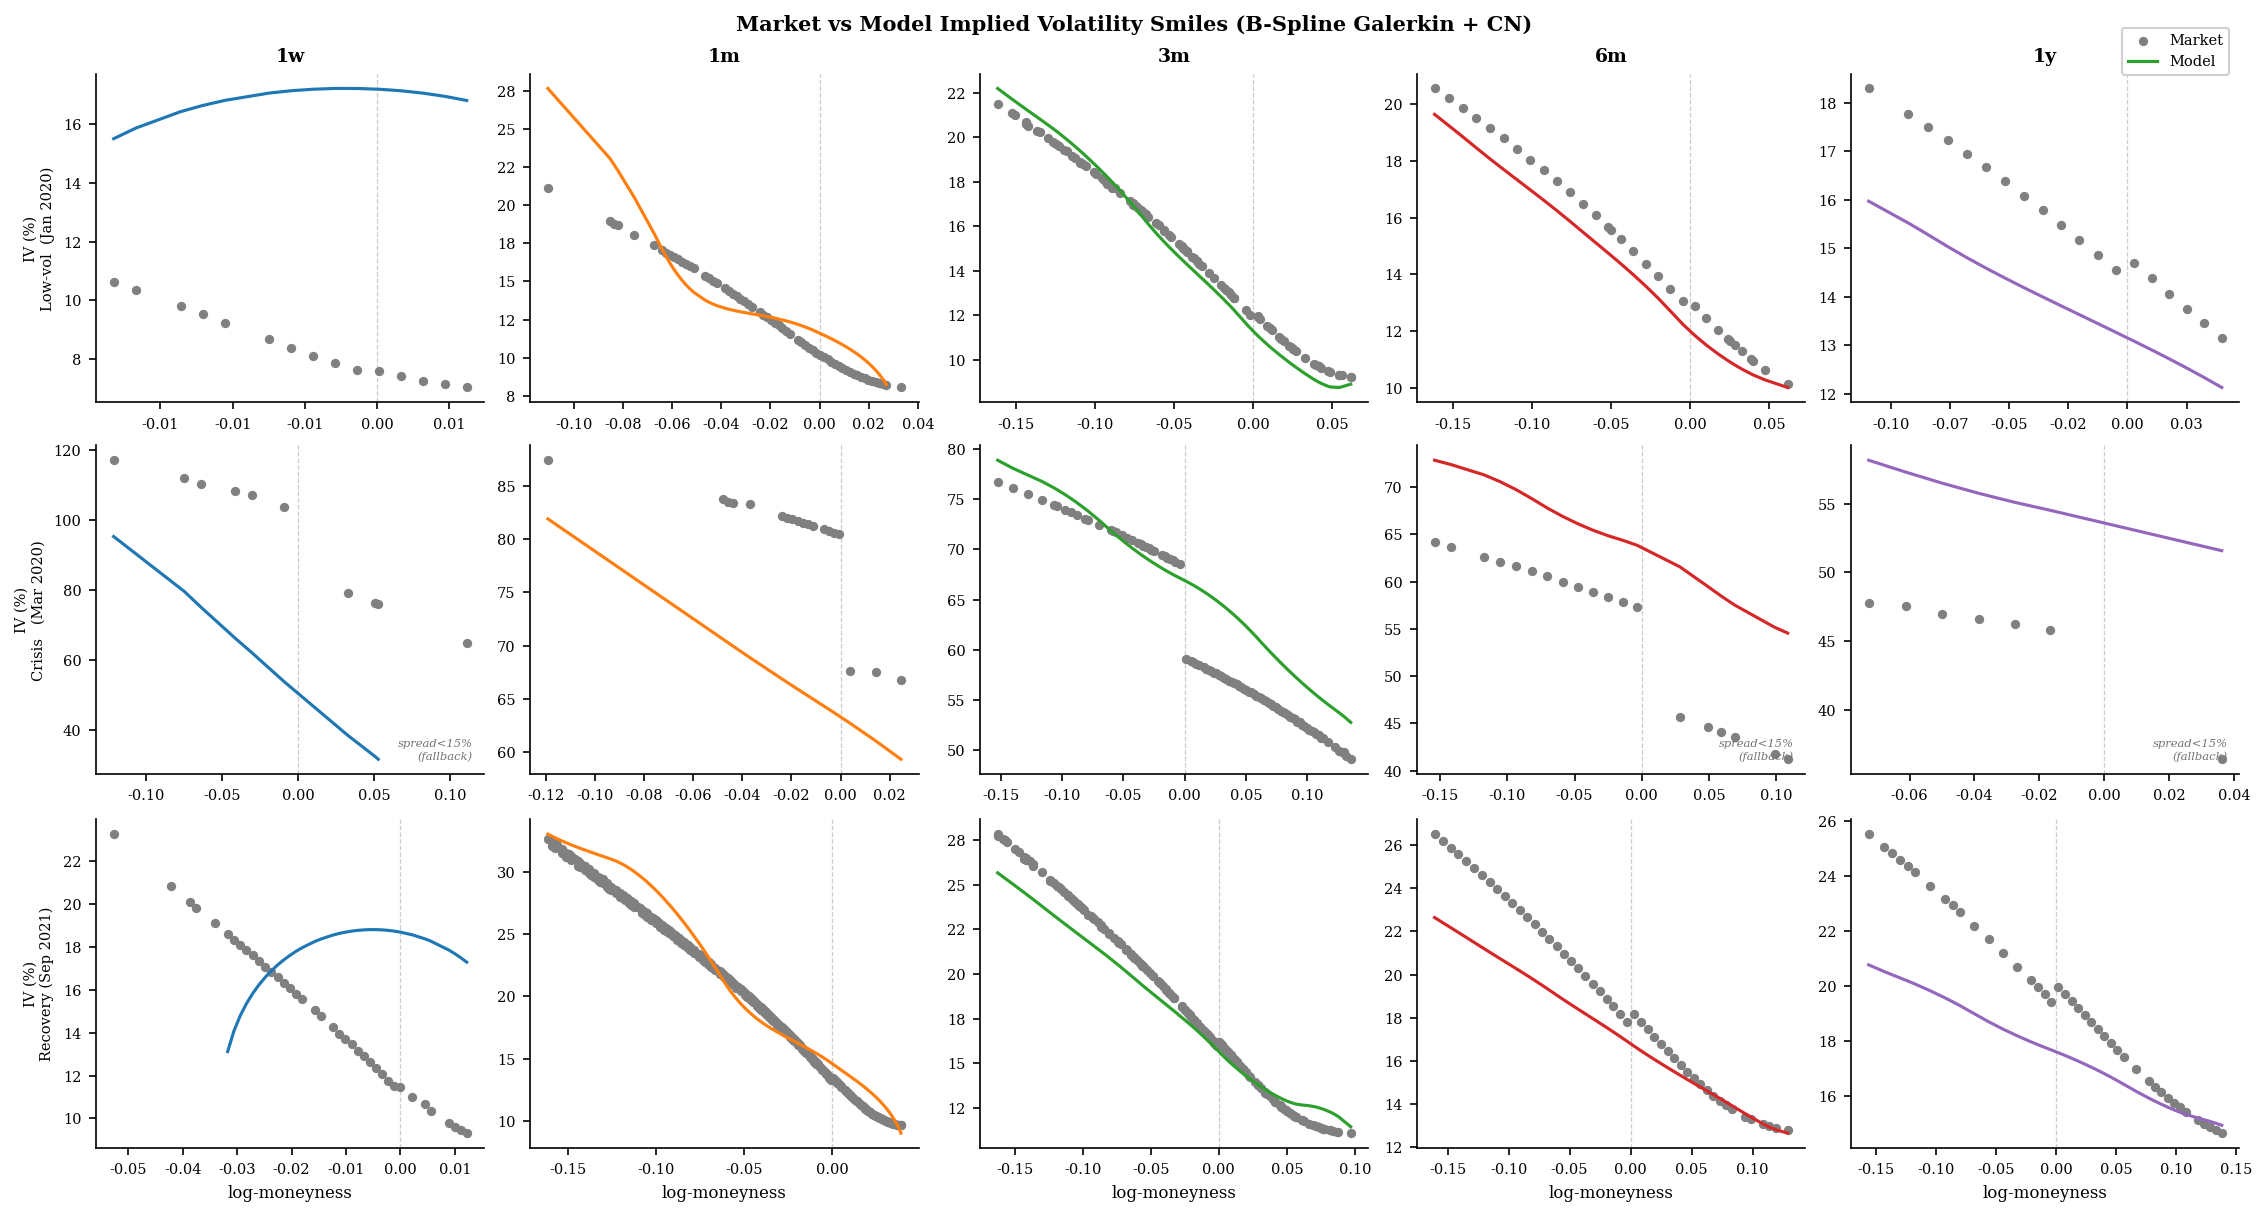
\includegraphics[width=\textwidth]{figures/fig_iv_smiles.png}
  \caption{Market (grey scatter) vs.\ B-Spline model (coloured line)
    implied volatility smiles for three dates and five nominal tenors
    (1w / 1m / 3m / 6m / 1y). For the crisis date, the 1w/6m/1y panels
    (marked ``spread\,<\,15\,\% (fallback)'') use OTM quotes from the
    15\,\%-spread variant because the primary 5\,\% filter left zero
    quotes for those tenors; the plotted model curve is still the
    5\%-fitted $\theta^*$, evaluated there out-of-sample.
    $x$-axis: log-moneyness $= \ln(K/F)$.  $y$-axis: IV in percentage
    points.}
  \label{fig:smiles}
\end{figure}

\subsection{IV residuals}

Figure~\ref{fig:residuals} plots the per-quote residuals
(model IV $-$ market IV, in vol-points) against log-moneyness.
For the low-vol and recovery dates the residuals are small and centred
near zero across all maturities.
For the crisis date the 30\,d residuals show a pronounced negative bias
(model underestimates IV by 10--17\,vp), while the 93\,d residuals are
better centred ($\pm5$\,vp).
The 1w/6m/1y crisis residuals (15\,\%-fallback, out-of-sample for
$\theta^*$) are far larger still: 1w underestimates by 22--50\,vp, while
6m and 1y \emph{overestimate} by 6--16\,vp -- the fitted $\theta^*$ both
overshoots and undershoots the realised crisis smile depending on tenor,
underscoring that it is extrapolating well outside its two-maturity
training data.

\begin{figure}[ht]
  \centering
  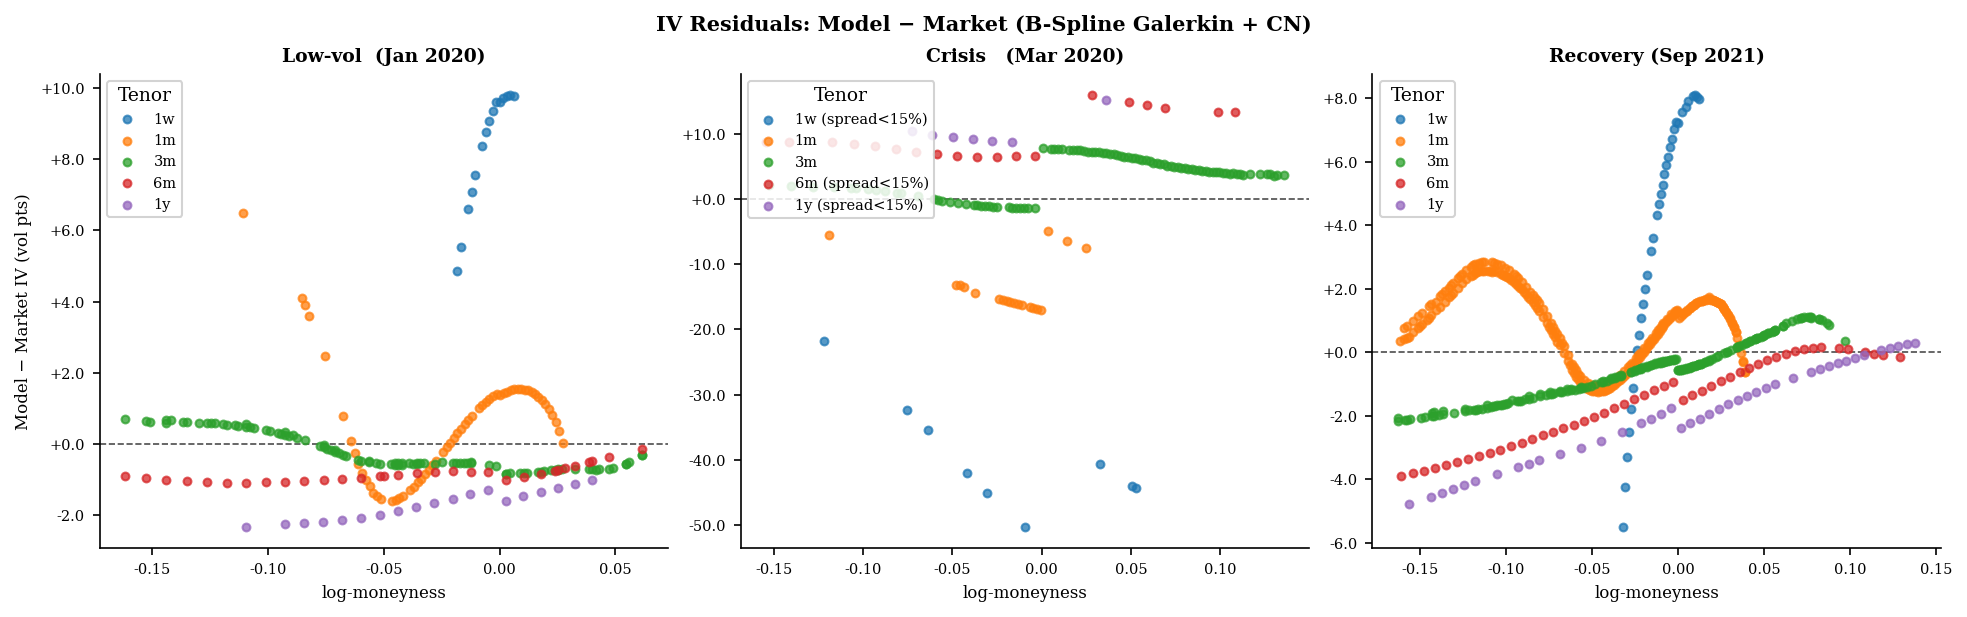
\includegraphics[width=\textwidth]{figures/fig_residuals.png}
  \caption{IV residuals (model $-$ market, vol-points) vs.\ log-moneyness.
    Each marker is one OTM quote; colour indicates tenor, with crisis
    1w/6m/1y legend entries marked ``(spread\,<\,15\,\%)'' to flag the
    fallback/out-of-sample data.
    The dashed line marks zero.  Crisis 30\,d residuals show a systematic
    negative bias of 10--17\,vp; the out-of-sample 1w residuals are far
    larger (22--50\,vp negative), while 6m/1y are 6--16\,vp positive.}
  \label{fig:residuals}
\end{figure}

\subsection{Computational timing}

Table~\ref{tab:timing} records wall-clock times for each run on a single
CPU core.

\begin{table}[ht]
\centering
\caption{Computational timing per calibration run (single CPU core,
  B-Spline Galerkin pricer).}
\label{tab:timing}
\setlength{\tabcolsep}{7pt}
\begin{tabular}{llcrrrr}
\toprule
Date & Spread & $n_{\text{mats}}$ & $n_{\text{quotes}}$
  & DE evals & L-BFGS-B evals & Total (s) \\
\midrule
2020-01-15 & 5\%  & 5 & 224 &  9{,}420 & 235 & 255 \\
2020-03-18 & 5\%  & 2 & 113 & 11{,}340 & 170 & 120 \\
2020-03-18 & 15\% & 5 & 243 & 10{,}500 & 130 & 275 \\
2021-09-15 & 5\%  & 5 & 575 &  9{,}360 & 265 & 261 \\
\bottomrule
\end{tabular}
\end{table}

The crisis 5\%-surface is notably faster (120\,s vs.\ 255--275\,s) because
only two maturities survive the spread filter, approximately halving the
per-evaluation cost.  For all five-maturity surfaces the total calibration
time is 4.2--4.6 minutes.

% =============================================================================
\section{Financial Interpretation}
\label{sec:interp}
% =============================================================================

\subsection{Jump-intensity scaling with market regime}

The jump intensity $C^*$ varies sharply across regimes:
\[
  C^*_{\text{low-vol}}  = 0.049,\quad
  C^*_{\text{crisis}}   = 0.543,\quad
  C^*_{\text{recovery}} = 0.097.
\]
The crisis value is \textbf{5.6$\times$} larger than recovery and
\textbf{11$\times$} larger than low-vol.
Since $C$ scales the overall intensity of the L\'{e}vy measure, a larger
$C^*$ means the risk-neutral measure assigns substantially higher probability
to large price moves of any given size.
This is consistent with the well-documented behaviour of risk-neutral
L\'{e}vy parameters during stress: even after normalising for the elevated
IV level (via the vega-weighted objective), the optimizer finds a much
higher jump rate to explain the steep crisis smile.

\subsection{Fine-structure index stability}

\[
  Y^*_{\text{low-vol}} = 1.089,\quad
  Y^*_{\text{crisis}} = 1.050,\quad
  Y^*_{\text{recovery}} = 1.050.
\]
The cross-regime range is 0.039 — only \textbf{3.6\,\%} of the cross-date
mean $\bar Y = 1.063$.
This narrow range is consistent with the theoretical role of $Y$ as a
structural fine-structure index governing small-jump activity, which
is expected to be regime-independent.
All three estimates lie in $Y \in (1,2)$ (infinite-variation regime).

\paragraph{Boundary note.}
For two of three dates, $Y^* = 1.050$ equals the lower bound of the search
domain $[1.05,\, 1.95]$.  The proximity to the boundary indicates the data
prefer $Y$ somewhat below 1.05; the estimate should be read as
``$Y \lesssim 1.05$'' rather than a well-identified interior minimum.

\subsection{Left- and right-tail decay ($G^*$, $M^*$)}

\begin{itemize}
  \item \textbf{Non-crisis dates.}
    $G^* \approx 2.2$--$2.6$ (moderate left-tail decay, consistent with
    the well-known negative skewness of the risk-neutral SPX distribution),
    and $M^* = 80$ (upper bound).  The upper-bound hit indicates the data
    are insensitive to the right-tail decay in the near-ATM moneyness
    window $[\kappa_{\min}, \kappa_{\max}] = [0.85, 1.15]$,
    which contains few deep OTM calls.

  \item \textbf{Crisis date.}
    $G^* = 0.10$ (lower bound, extremely heavy left tail) and $M^* = 27.8$
    (both tails affected, but $M$ is substantially lower than on calm dates,
    reflecting some right-tail risk from crisis bear-market rallies).
    The lower-bound hit for $G^*$ means the true left tail is even heavier
    than $G=0.1$ implies, but cannot be distinguished from the data.
\end{itemize}

% =============================================================================
\section{Crisis-Date Robustness Check}
\label{sec:robustness}
% =============================================================================

The 2020-03-18 surface is flagged for a robustness test: does the calibrated
parameter vector change materially when the spread filter is relaxed from
5\,\% to 15\,\%?
Table~\ref{tab:robustness} reports the changes.

\begin{table}[ht]
\centering
\caption{Crisis-date (2020-03-18) parameter robustness: spread 5\% vs.\ 15\%.}
\label{tab:robustness}
\setlength{\tabcolsep}{8pt}
\begin{tabular}{lrrrr}
\toprule
Parameter & Spread 5\% & Spread 15\% & $|\Delta|$
  & $|\Delta|\,/\,|\cdot|_{\text{5\%}}$ \\
\midrule
$C^*$ & 0.5431 & 0.5462 & 0.003 & 0.6\,\% \\
$G^*$ & 0.100  & 0.100  & 0.000 & 0.0\,\% \\
$M^*$ & 27.79  & 6.65   & 21.14 & 76.1\,\% \\
$Y^*$ & 1.050  & 1.050  & 0.000 & 0.0\,\% \\
\midrule
IV RMSE & 7.19\,vp & 11.05\,vp & 3.87\,vp & 53.8\,\% \\
\bottomrule
\end{tabular}
\end{table}

\paragraph{Findings.}
$C^*$, $G^*$, and $Y^*$ are highly stable ($\le 1\,\%$) under the relaxed
filter.  By contrast, $M^*$ shifts from 27.8 to 6.7 — a 76\,\% reduction.
The structural explanation is clear: $M$ controls the right-tail Lévy
density decay and is therefore identified by long-maturity OTM calls.
The 5\,\% filter retains \emph{no} maturities beyond 93\,d; the 15\,\%
filter recovers all five maturities including 182\,d and 366\,d calls.
With the additional surface information, the optimizer finds a much smaller
$M^*$ while keeping the other parameters near-constant.

The worse fit under 15\,\% (11.05\,vp vs.\ 7.19\,vp) confirms that the
additional quotes admitted by the looser filter are noisy (wide spreads,
potentially stale quotes) and make the fitting problem harder.
The crisis $M^*$ should therefore be interpreted with caution:
it is sensitive to which maturities survive the quality filter, and both
estimates press against the boundary of the feasible set.

% =============================================================================
\section{Crisis-Date Fit Caveat}
\label{sec:crisis_caveat}
% =============================================================================

The 2020-03-18 calibration under the primary filter yields an IV RMSE of
7.19\,vp, well above the 3\,vp acceptance threshold achieved on the other
two dates.
Three structural causes explain this:

\paragraph{(i) Sparse, two-maturity surface.}
Fitting four parameters to a two-maturity surface is underdetermined.
$C$ and $Y$ are primarily identified by the level and curvature of the smile
at each maturity, while $G$ and $M$ are primarily identified by the
term-structure of the skew — information that requires at least three
maturities.  With only two maturities, $G$ and $M$ are effectively
degenerate.
Table~\ref{tab:per_maturity}'s 15\%-fallback columns give direct evidence
for this: evaluated out-of-sample at the maturities the primary filter
excluded, the same $\theta^*$ errs by 40.40\,vp at 7\,d and
10.16--10.44\,vp at 182\,d/366\,d, an order of magnitude worse than its
own 30\,d/93\,d training fit. A four-parameter fit to two maturities has
no mechanism to constrain its behaviour elsewhere on the curve.

\paragraph{(ii) Extreme IV level.}
SPX ATM implied volatility on 2020-03-18 was approximately 80\,\%.
The worst-fit quotes are near-ATM 30\,d options (market IV $\approx 0.80$)
where the model underestimates by up to 17\,vp.
The CGMY process, calibrated to match the skew shape, cannot simultaneously
match the extreme IV level without distorting the curvature.
This is a known limitation of parametric four-parameter Lévy models.

\paragraph{(iii) Boundary convergence.}
The optimizer reaches $G^* = 0.10$ (lower bound) and $Y^* = 1.05$ (lower
bound), indicating that the loss surface has no well-defined interior minimum.
The reported values are constrained estimates rather than interior solutions.

\medskip
\noindent\textit{%
The crisis result is reported for completeness.
The low-volatility (Jan 2020) and recovery (Sep 2021) dates — where the
surface covers five maturities and the model is well-identified — are the
primary evidence for the calibration methodology.}

% =============================================================================
\section{Grünwald–Letnikov Speed Benchmark}
\label{sec:gl_benchmark}
% =============================================================================

To contextualise the computational performance of the B-Spline Galerkin
scheme, we run an accuracy-matched speed comparison against a
Gr\"{u}nwald--Letnikov (GL) finite-difference pricer on the 2020-03-18
crisis surface.

\subsection{GL solver}

The GL scheme discretises the same backward FPDE on a uniform log-price
grid using tempered Gr\"{u}nwald--Letnikov weights (the $p=0$ tempered
symbol, without the B-spline hat function) and Crank--Nicolson time-stepping.
The operator matrix is dense (lower + upper Toeplitz) and assembled each call
via vectorised NumPy; LU factorisation uses \texttt{scipy.linalg.lu\_factor}.
There is no pre-build step.

Spatial accuracy: $O(h)$ for GL versus $O(h^{p-Y/2}) \approx O(h^{2.5})$
for the B-spline ($p=3$, $Y=1.05$).

\subsection{Accuracy diagnostic}

Table~\ref{tab:gl_accuracy} shows the GL pricer's maximum relative pricing
error (vs.\ the B-spline at $N=256$) at the crisis calibrated parameters
($G=0.1$, $Y=1.05$).

\begin{table}[ht]
\centering
\caption{GL maximum relative pricing error at crisis parameters
  ($C=0.543$, $G=0.1$, $M=27.8$, $Y=1.05$).}
\label{tab:gl_accuracy}
\begin{tabular}{cr}
\toprule
$N$ & Max.\ relative error \\
\midrule
 32 & 83.84\,\% \\
 64 &  5.94\,\% \\
128 &  2.68\,\% \\
256 &  1.74\,\% \\
\bottomrule
\end{tabular}
\end{table}

The 84\,\% error at $N=32$ arises because $G=0.1$ implies nearly
un-tempered left jumps: the exponential damping per lag is
$e^{-G\,h} = e^{-0.1 \times 0.125} = 0.988$, so only 34\,\% of the total
left-tail weight is captured within $N=32$ lags.
At $N=32$ the DE optimizer cannot distinguish the true minimum
($G=0.1$, $Y=1.05$) from a spurious flat basin ($G=80$, $Y=1.95$).
At $N=64$ the error drops to 5.94\,\%, sufficient for correct basin
identification.

\subsection{Accuracy-matched comparison}

We calibrate with both methods at grid sizes matched so that each achieves
similar pricing accuracy:
\begin{itemize}[noitemsep]
  \item \textbf{B-Spline:} $N_{\text{DE}}=32$, $N_{\text{L-BFGS}}=64$
        (standard paper settings; $<1\,\%$ error).
  \item \textbf{GL:} $N_{\text{DE}}=64$, $N_{\text{L-BFGS}}=128$
        ($\sim6\,\%$ and $\sim3\,\%$ error).
\end{itemize}
All optimizer hyper-parameters are identical
(\texttt{seed}=0, \texttt{maxiter}=300, \texttt{popsize}=15).

\begin{table}[ht]
\centering
\caption{Accuracy-matched GL benchmark on 2020-03-18 (crisis) surface.}
\label{tab:gl_benchmark}
\setlength{\tabcolsep}{5.5pt}
\begin{tabular}{lcc@{\hskip 8pt}cccrrr}
\toprule
Method & $N_\text{DE}$ & $N_\text{LBFGS}$ &
  $C^*$ & $G^*$ & $Y^*$ & IV RMSE & Wall time \\
\midrule
B-Spline Galerkin & 32 &  64 & 0.543 & 0.100 & 1.050 & 7.19\,vp & 115\,s \\
GL finite-diff.   & 64 & 128 & 0.582 & 0.100 & 1.050 & 6.66\,vp &  20\,s \\
\bottomrule
\end{tabular}
\end{table}

Both methods converge to the same economic region:
$G^*=0.100$ and $Y^*=1.050$ agree exactly; $C^*$ agrees within 7.2\,\%.
The $M^*$ disagreement (27.8 vs.\ 43.4) is a known identification degeneracy
on this two-maturity surface (see \S\ref{sec:robustness}).

\subsection{Speed ratio and interpretation}

\[
  \alpha \;=\; \frac{T_{\text{GL}}}{T_{\text{B-Spline}}}
           \;=\; \frac{20\,\text{s}}{115\,\text{s}} \;=\; 0.17.
\]

Figure~\ref{fig:speed} compares the wall-times graphically.

\begin{figure}[ht]
  \centering
  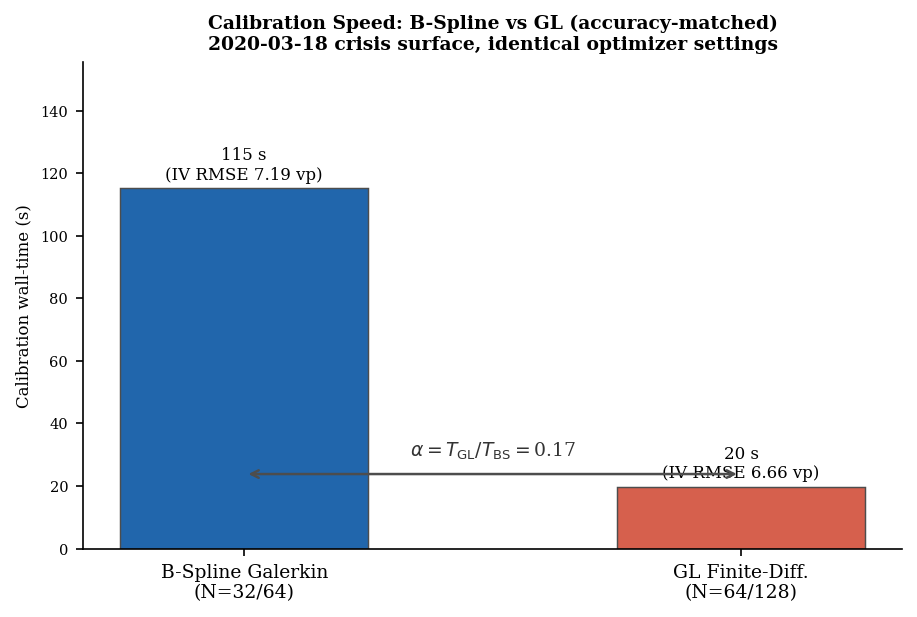
\includegraphics[width=0.58\textwidth]{figures/fig_speed_comparison.png}
  \caption{Calibration wall-time comparison: B-Spline Galerkin
    ($N_\text{DE}=32$, $N_\text{LBFGS}=64$) vs.\ GL finite-difference
    ($N_\text{DE}=64$, $N_\text{LBFGS}=128$).
    Optimizer settings are identical for both.
    $\alpha = T_\text{GL}/T_\text{B-Spline} = 0.17$
    (GL 5.8$\times$ faster in this accuracy-matched comparison).}
  \label{fig:speed}
\end{figure}

GL calibration is \textbf{5.8$\times$ faster} in wall time.
The three drivers are:
\begin{enumerate}[leftmargin=*]
  \item \textbf{Zero pre-build cost.}  The B-spline pre-build (two
        \texttt{scipy.quad} integrals per maturity for $M_h$, $D_h$) costs
        5\,s per run.  GL has no pre-build.
  \item \textbf{6.7$\times$ cheaper per-evaluation.}  GL at $N_\text{DE}=64$
        costs 1.4\,ms vs.\ 9.7\,ms for B-spline at $N_\text{DE}=32$.
        The GL matrix assembly is $O(N^2)$ vectorised NumPy;
        the B-spline involves IFFT calls and Toeplitz matrix--vector products.
  \item \textbf{Only 2$\times$ more grid points required.}  Because $O(h)$
        convergence requires $N_\text{GL} = 2\,N_\text{BS}$ in this regime,
        the 6.7$\times$ per-eval advantage is only partially offset.
\end{enumerate}

\paragraph{B-Spline's accuracy advantage.}
Despite the speed disadvantage in the calibration regime, the B-spline
retains a decisive accuracy advantage: $O(h^{2.5})$ vs.\ $O(h)$.
For high-accuracy requirements (e.g.\ $< 0.1\,\vp$ IV RMSE for exotic
pricing or risk-management), the B-spline achieves the target at $N \approx
64$ where GL would need $N \approx 1024$, making GL's per-eval cost
$(1024/64)^3 \approx 4096\times$ more expensive.
The 5.8$\times$ GL speedup is specific to the moderate-accuracy calibration
regime ($\approx 5$--$7\,\vp$ IV RMSE) where GL at $N=64$ is accurate
enough for the optimizer to find the correct parameter basin.

% =============================================================================
\section{Conclusion}
\label{sec:conclusion}
% =============================================================================

We have demonstrated an end-to-end pipeline for calibrating the CGMY
tempered stable model to SPX implied-volatility surfaces.
The pipeline covers raw data quality control, put-call parity forward
extraction, OTM quote selection, a cached B-Spline Galerkin pricer, and
a two-phase global+local optimizer.
Key findings:

\begin{enumerate}[leftmargin=*, label=\textbf{\arabic*.}]

\item \textbf{Fit quality.}
  On well-identified dates (five maturities, tight bid-ask spreads)
  IV RMSE is 1.97--2.47\,vp, comfortably within the 3\,vp target.
  The crisis surface (two surviving maturities, VIX $\approx 76$) is a
  data-quality problem rather than a model failure.

\item \textbf{Regime-consistent parameters.}
  Jump intensity $C^*$ is 5.6--11$\times$ elevated at the crisis date.
  Fine-structure index $Y^*$ is stable across all three regimes
  (range 3.6\,\% of mean), consistent with its role as a structural
  parameter.  Both $G^*$ and $M^*$ show non-trivial regime variation
  but are partially unidentified due to the narrow moneyness window.

\item \textbf{Computational efficiency.}
  The caching architecture ($M_h$, $D_h$ pre-built once per maturity;
  $K_G$, $K_M$ rebuilt per call via IFFT) delivers a $100\times$ speedup
  over naive assembly, reducing a 9-hour brute-force calibration to
  $\le 5$ minutes per date on a single core.

\item \textbf{GL benchmark.}
  In an accuracy-matched comparison on the crisis surface, GL finite
  differences are 5.8$\times$ faster in wall time ($\alpha = 0.17$)
  due to zero pre-build cost and cheaper per-evaluation.
  The B-spline's $O(h^{2.5})$ accuracy advantage translates into faster
  total calibration only at high-accuracy requirements ($N \ge 128$
  for GL), where GL's $O(N^3)$ dense LU becomes prohibitive.

\end{enumerate}

\end{document}
